\section{Introduction}
\label{sec:intro}

Effective performance monitoring of large networks is crucial to quickly
localize problems like high queueing latency~\cite{int}, TCP
incast~\cite{tcpincast}, and load imbalance across network links~\cite{conga}.
A common approach to network monitoring is to collect information from the
endpoint network stack~\cite{minlan-snap, pathdump, trumpet} or
to use end-to-end probes~\cite{pingmesh} to diagnose performance problems.  While
endpoints provide application context, they lack visibility to localize
performance problems at links deep in the network. For example, it is
challenging to localize queue buildup to a particular switch or pinpoint
traffic causing the queue buildup, forcing operators to infer the network-level
root causes indirectly~\cite{pingmesh}.

Switch-based monitoring could allow operators to diagnose problems with more
direct visibility into performance statistics. However, traditional switch
mechanisms like sampling~\cite{netflow, sflow}, mirroring~\cite{cisco-span,
netsight, everflow}, and counting~\cite{cormode, univmon} are quite restrictive.  Sampling
and mirroring miss events of interest as it is infeasible to collect
information on all packets, while counters only track traffic volume
statistics. None of these mechanisms provides relevant performance data, like
queueing delays.

Some upcoming technologies recognize the need for better performance monitoring
using switches. In-band network telemetry~\cite{int} writes queueing delays
experienced by a packet on the packet itself, allowing endpoints to localize
delay spikes. The Tetration switching chip~\cite{tetration-telemetry} provides
a flow cache that measures flow-level performance metrics.  These metrics are
useful, but they are exposed at a fixed granularity (\eg per 5-tuple), and the metrics themselves
are fixed. For example, the list of exposed metrics includes flow-level latency
and packet size variation, but not latency variation, \ie jitter.

Operator requirements are ever-changing, and redesigning hardware is expensive.
We believe that the trajectory of adding fixed-function switch monitoring
piecemeal is unsustainable. Instead, we advocate building performance
monitoring primitives that can be flexibly reused for a variety of
needs. Programmable switches~\cite{flexpipe, tofino, xpliant} now support flexible
parsing~\cite{gibb_parsing}, header processing~\cite{rmt, domino_sigcomm}, and
scheduling~\cite{pifo_sigcomm}. Our goal is to add monitoring to this list.

This paper applies {\em language-directed hardware design} to the problem of
flexible performance monitoring, inspired by early efforts on designing
hardware to support high-level
languages~\cite{language-directed-computer-design, ditzel_patterson, soar}.
Specifically, we design a language that can express a broad variety of
performance monitoring use cases, and then design high-speed switch hardware
primitives in service of this language. By designing hardware to support an
expressive language, we believe the resulting hardware design can support a
wide variety of current and future performance monitoring needs.

\begin{figure}[!t]
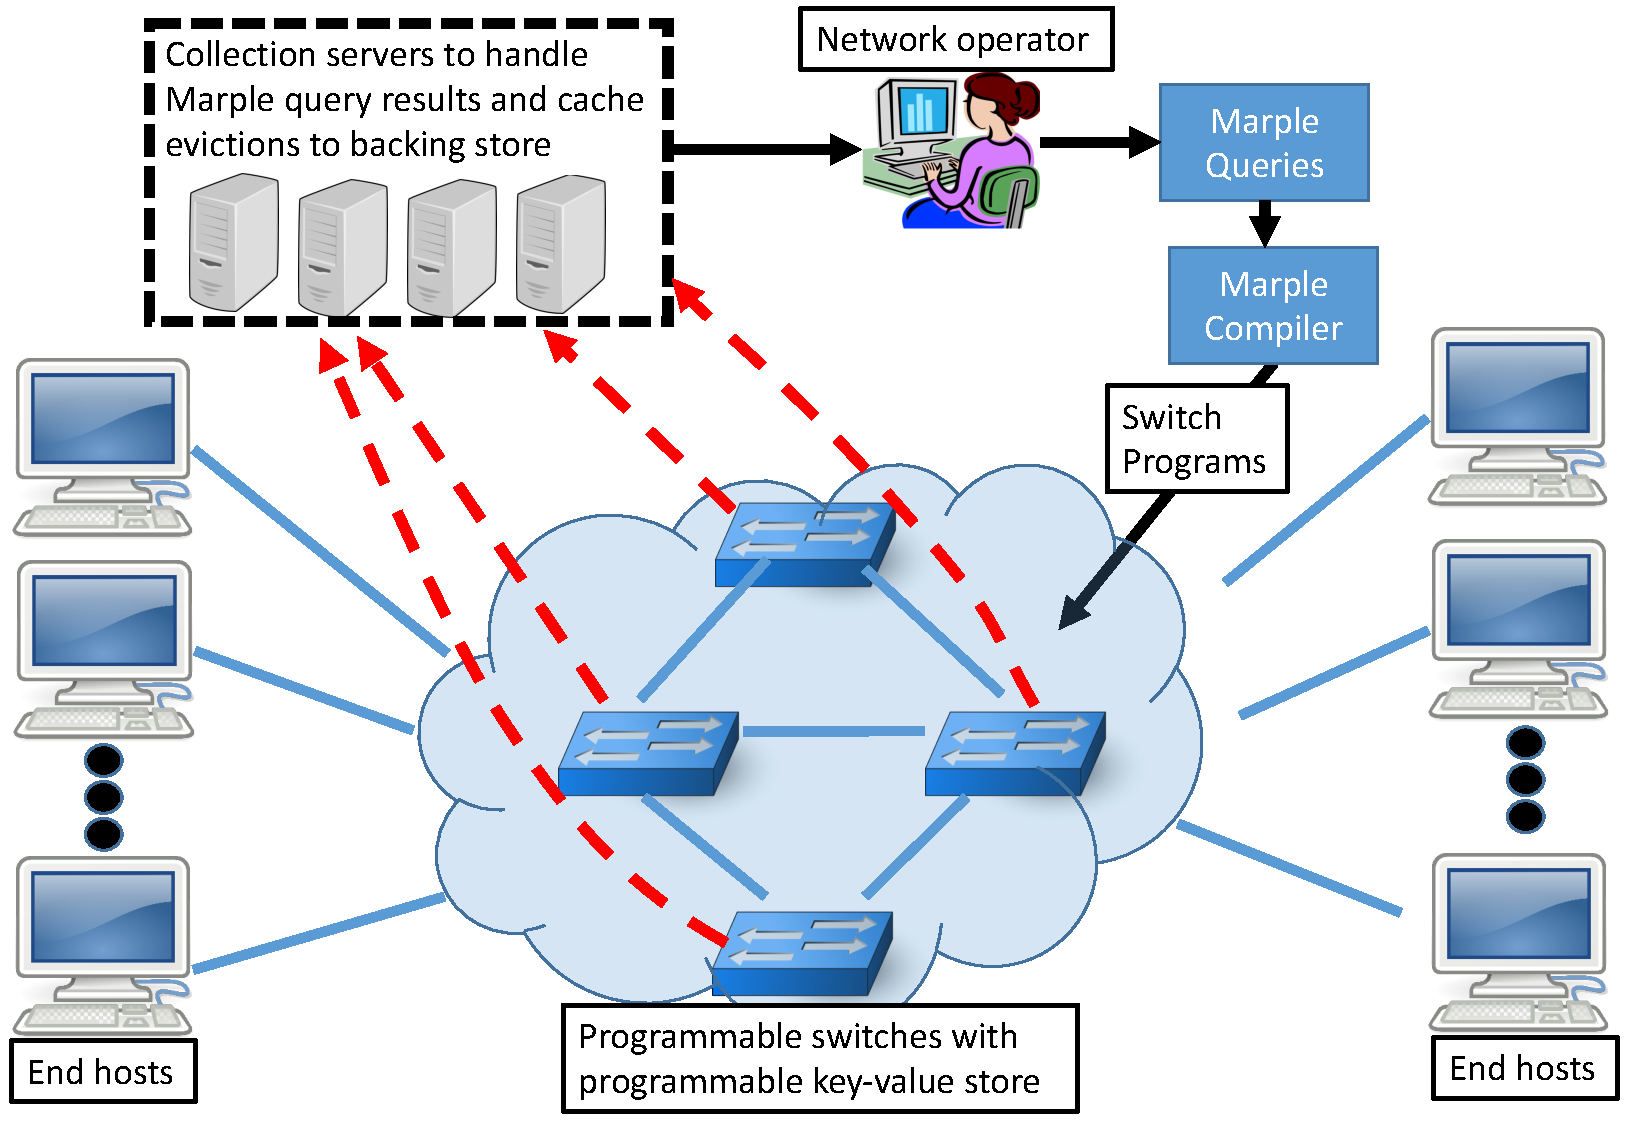
\includegraphics[width=\columnwidth]{pq_overview.pdf}
\caption{Operators issue \TheSystem queries, which are compiled into switch
programs for programmable switches augmented with our new programmable
key-value store primitive. Switches stream results from this query to
collection servers that also house the backing store for the key-value store.}
\label{fig:overview}
\end{figure}

\Fig{overview} provides an overview of our performance monitoring system. To
use the system, an operator writes a query in a domain-specific language called
{\em \TheSystem,} either to implement a long-running monitor for a statistic (\eg
detecting TCP timeouts), or to troubleshoot a specific problem (\eg incast~\cite{tcpincast}) at hand. The
query is compiled into a switch program that runs on the network's programmable
switches, augmented with new switch hardware primitives that we design in
service of \TheSystem.  The switches stream results out to collection servers,
where the operator can retrieve query results. We now briefly describe the
three components of our system: the query language, the switch hardware, and
the query compiler.

\Para{Performance query language.} \TheSystem uses familiar functional
constructs like {\ct map}, {\ct filter}, {\ct groupby} and {\ct zip} for
performance monitoring.
\TheSystem provides the abstraction of a stream that contains performance
information for {\em every packet at every queue} in the network
(\Sec{language}).
%
Programmers can focus their attention on traffic experiencing interesting
performance using {\ct filter} (\eg packets with high queueing latencies),
aggregate information across packets in flexible ways using {\ct groupby} (\eg
compute a moving average over queueing latency per flow), compute new stateless
quantities using {\ct map} (\eg binning a packet's timestamp into an epoch), and
detect simultaneous performance conditions using {\ct zip} (\eg when the queue
depth is large and the number of connections in the queue is high).

\Para{Hardware design for performance queries.} 
A \naive implementation of \TheSystem might stream every packet's
metadata from the network to a central location and run streaming queries
against it. Modern scale-out data-processing systems support ~100K--1M
operations per second per core~\cite{kafka_benchmark, redis_benchmark,
memcached_benchmark, redis_vs_memcached_update,
spark-streaming}, but processing every single packet (assuming a relatively
large packet size of 1 KB) from a single 1 Tbit/s switch would need ~100M
operations per second --- 2--3 orders of magnitude more than what existing systems
support.

Instead, we leverage high-speed programmable switches~\cite{rmt, xpliant,
tofino, flexpipe} as first-class citizens in network monitoring, because they
can programmatically manipulate multi-Tbit/s packet streams.  Early filtering
and flexible aggregation on switches drastically reduce the number of records per
second streamed out to a standard data-processing system running on
the collection server.

While programmable switches support many of \TheSystem's stateless
language constructs that modify packet fields alone (\eg {\ct map} and {\ct
filter}), they do not support aggregation of state across packets for a large
number of flows (\ie {\ct groupby}). To support flexible aggregations over
packets, we design a
programmable key-value store in hardware (\Sec{aggregation}), where the keys
represent flow identifiers and the values represent the state computed by the
aggregation function. This key-value store must
update values at the line rate of 1 packet per clock cycle (at 1
GHz~\cite{rmt, xpliant_sdk}) and support millions of keys (\ie flows).
Unfortunately, neither SRAM nor DRAM is simultaneously fast and dense
enough to meet both requirements.

We split the key-value store into a small but fast on-chip cache in SRAM and a
larger but slower off-chip backing store in DRAM. Traditional caches incur
variable write latencies due to cache misses; however, line-rate packet
forwarding requires deterministic latency guarantees. Our design accomplishes
this by never reading back a value into the cache if it has already been
evicted to the backing store. Instead, it treats a cache miss as the arrival of
a packet from a new flow. When a flow is evicted, we {\em merge} the evicted flow's value in the cache with the flow's
old value in the backing store. Because merges occur off the
critical packet processing path, the backing store can be implemented in
software on a separate collection server.% or on off-chip DRAM on the switch.

While it is not always possible to merge an aggregation function without losing
accuracy, we characterize a class of affine aggregation functions, which we
call {\em linear-in-state}, for which accurate merging is possible.  Many
useful aggregation functions are linear-in-state, \eg counters, predicated
counters (\eg count only TCP packets that saw timeouts), exponentially weighted
moving averages, and functions computed over a finite window of packets.  We
design a switch instruction to support linear-in-state functions, finding that
it easily meets timing at 1 GHz, while occupying modest silicon area.

\Para{Query compiler.} We implement a compiler that takes \TheSystem queries
and compiles them into switch configurations for two targets (\Sec{compiler}):
(1) the P4 behavioral model~\cite{p4-bmv2}, an open source programmable
software switch that can be used for end-to-end evaluations of \TheSystem on
Mininet~\cite{mininet}, and (2) Banzai~\cite{domino_sigcomm}, a simulator for high-speed
programmable switch hardware that can be used to experiment with different instruction sets.
The \TheSystem compiler detects linear-in-state aggregations in input queries
and successfully targets the linear-in-state switch instruction that we add to
Banzai.

\Para{Evaluation.} We show that \TheSystem can express a variety of useful
performance monitoring examples, like detecting and localizing TCP incast and
measuring the prevalence of out-of-order TCP packets. \TheSystem queries
require between 4 and 11 pipeline stages, which is modest for a 32-stage switch
pipeline~\cite{rmt}. We evaluate our key-value store's performance using
trace-driven simulations. For a 64 Mbit on-chip cache, which occupies about
10\% of the area of a \tengswitch switching chip, we estimate that the cache eviction rate
from a single top-of-rack switch can be handled by a single 8-core server running
Redis~\cite{redis}.
We evaluate \TheSystem's usability through two Mininet case studies
that use \TheSystem to troubleshoot high tail latencies~\cite{barefoot-demo} and
measure the distribution of flowlet sizes~\cite{conga}. \TheSystem is open
source and available at \url{http://web.mit.edu/marple}.
